\documentclass{standalone}
\usepackage{tikz}

\begin{document}

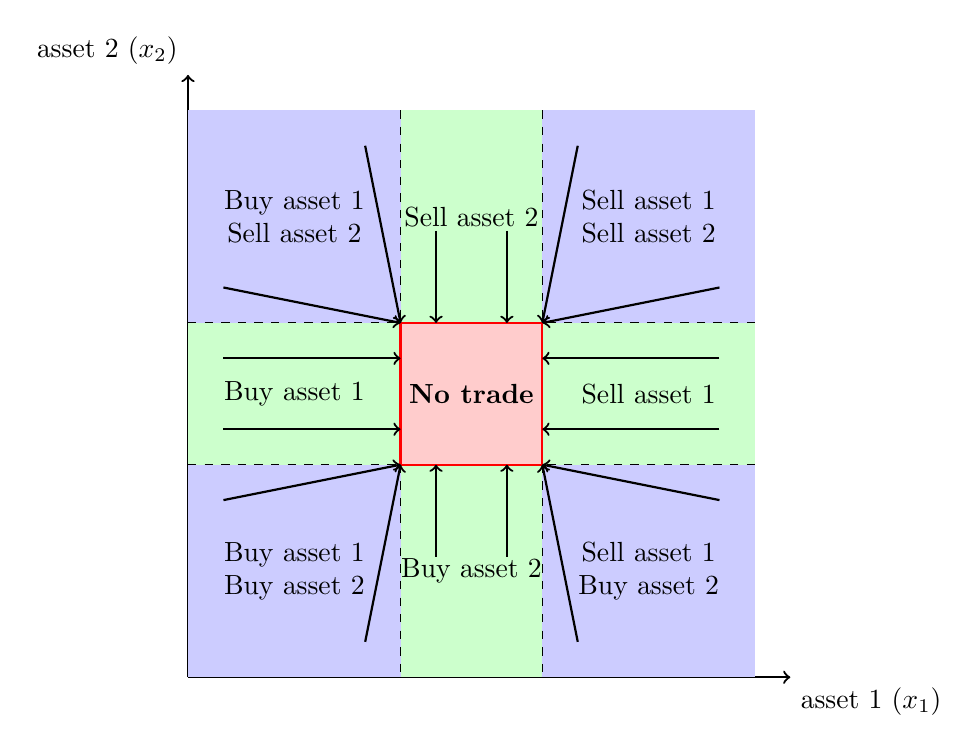
\begin{tikzpicture}[scale=0.9] % Reduced scale for a smaller plot

    % Draw axes
    \draw[->, thick] (-4, -4) -- (4.5, -4) node[below right] {asset 1 (\(x_1\))};
    \draw[->, thick] (-4, -4) -- (-4, 4.5) node[above left] {asset 2 (\(x_2\))};

    % Blue regions (squares)
    \fill[blue!20] (-4, 1) rectangle (-1, 4); % Top-left
    \fill[blue!20] (1, 4) rectangle (4, 1);  % Top-right
    \fill[blue!20] (1, -1) rectangle (4, -4); % Bottom-right
    \fill[blue!20] (-4, -4) rectangle (-1, -1); % Bottom-left

    % Green regions (squares between blue regions)
    \fill[green!20] (-1, 1) rectangle (1, 4); % Top (between blue regions)
    \fill[green!20] (-4, -1) rectangle (-1, 1); % Left (between blue regions)
    \fill[green!20] (1, -1) rectangle (4, 1); % Right (between blue regions)
    \fill[green!20] (-1, -4) rectangle (1, -1); % Bottom (between blue regions)

    % No-Trade Region (NTR) - Red Square
    \filldraw[fill=red!20, draw=red, thick] (-1, -1) rectangle (1, 1);
    \node at (0, 0) {\textbf{No trade}};

    % Labels for blue regions
    \node[align=center] at (-2.5, 2.5) {Buy asset 1\\Sell asset 2};
    \node[align=center] at (2.5, 2.5) {Sell asset 1\\Sell asset 2};
    \node[align=center] at (2.5, -2.5) {Sell asset 1\\Buy asset 2};
    \node[align=center] at (-2.5, -2.5) {Buy asset 1\\Buy asset 2};

    % Labels for green regions
    \node at (0, 2.5) {Sell asset 2};
    \node at (-2.5, 0) {Buy asset 1};
    \node at (2.5, 0) {Sell asset 1};
    \node at (0, -2.5) {Buy asset 2};

    % Diagonal dashed lines for each blue region, closer to NTR (third diagonal)
    % Top-left blue region
    \draw[dashed] (-1, 4) -- (-1, 1); % Vertical closer to NTR
    \draw[dashed] (-4, 1) -- (-1, 1); % Horizontal closer to NTR

    % Top-right blue region
    \draw[dashed] (1, 4) -- (1, 1); % Vertical closer to NTR
    \draw[dashed] (4, 1) -- (1, 1); % Horizontal closer to NTR

    % Bottom-right blue region
    \draw[dashed] (1, -1) -- (1, -4); % Vertical closer to NTR
    \draw[dashed] (4, -1) -- (1, -1); % Horizontal closer to NTR

    % Bottom-left blue region
    \draw[dashed] (-1, -1) -- (-1, -4); % Vertical closer to NTR
    \draw[dashed] (-4, -1) -- (-1, -1); % Horizontal closer to NTR

    % Arrows for trade directions (two arrows per box, pointing to NTR boundary)
    % Top-left region (blue)
    \draw[->, thick] (-1.5, 3.5) -- (-1, 1); % Existing diagonal
    \draw[->, thick] (-3.5, 1.5) -- (-1, 1); % Existing diagonal

    % Top-right region (blue)
    \draw[->, thick] (1.5, 3.5) -- (1, 1); % Existing diagonal
    \draw[->, thick] (3.5, 1.5) -- (1, 1); % Existing diagonal

    % Bottom-right region (blue)
    \draw[->, thick] (3.5, -1.5) -- (1, -1); % Existing diagonal
    \draw[->, thick] (1.5, -3.5) -- (1, -1); % Existing diagonal

    % Bottom-left region (blue)
    \draw[->, thick] (-1.5, -3.5) -- (-1, -1); % Existing diagonal
    \draw[->, thick] (-3.5, -1.5) -- (-1, -1); % Existing diagonal

    % Top region (green)
    \draw[->, thick] (-0.5, 2.3) -- (-0.5, 1); % Vertical to top of NTR
    \draw[->, thick] (0.5, 2.3) -- (0.5, 1); % Vertical to top of NTR

    % Right region (green)
    \draw[->, thick] (3.5, 0.5) -- (1, 0.5); % Horizontal to right of NTR
    \draw[->, thick] (3.5, -0.5) -- (1, -0.5); % Horizontal to right of NTR

    % Bottom region (green)
    \draw[->, thick] (-0.5, -2.3) -- (-0.5, -1); % Vertical to bottom of NTR
    \draw[->, thick] (0.5, -2.3) -- (0.5, -1); % Vertical to bottom of NTR

    % Left region (green)
    \draw[->, thick] (-3.5, -0.5) -- (-1, -0.5); % Horizontal to left of NTR
    \draw[->, thick] (-3.5, 0.5) -- (-1, 0.5); % Horizontal to left of NTR

\end{tikzpicture}

\end{document}